%!TEX root = nextndnvideo-tr.tex
\vspace{0.3cm}
\section{design} % (fold)
\label{sec:design}
\subsection{Architecture}
Next-NDNVideo is based on Consumer / Producer API over Named Data Networking. It contains two kinds of roles - producer and consumer. The whole architecture (Figure~\ref{fig:arch}) is described below.

\begin{figure*}%[htbp]
  \centering
  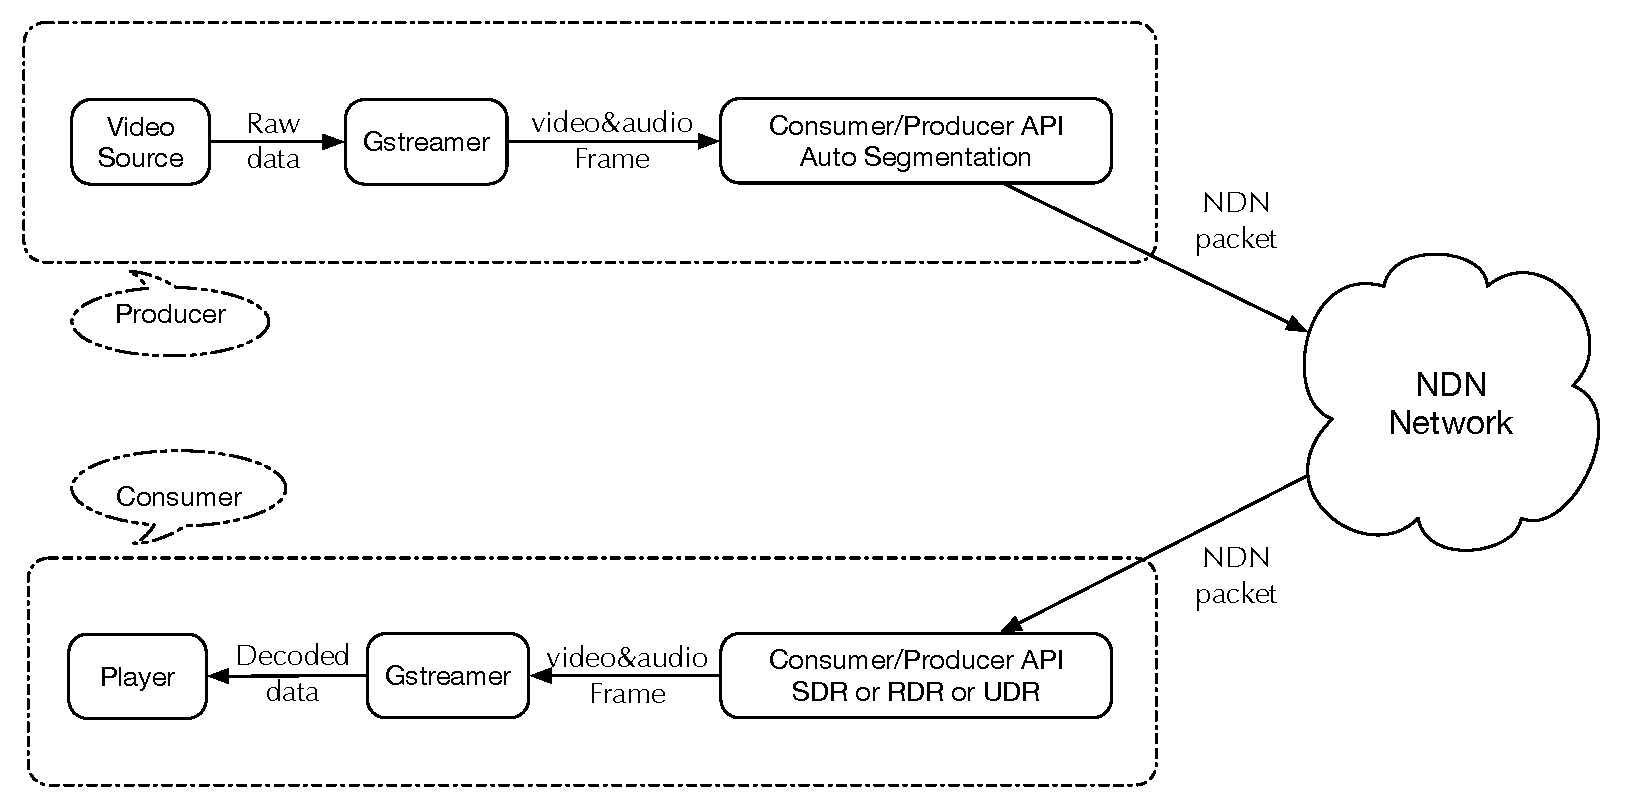
\includegraphics[scale=0.55]{architecture}
  % \vspace{-0.3cm}
  \caption{Architecture of Next-NDNVideo}
  \label{fig:arch}
  %\vspace{-0.2cm}
\end{figure*}

The producer is responsible for generating video and audio streaming. It behaves as the content publisher. We use Gstreamer to extract the video and audio frames from video source. Then we call Consumer / Producer API to encapsulate the data frames into NDN packets. In this case these NDN packets are available to fetch. The producer part can work even without being attached to the NDN network. The producer's packages will be cached in the \textit{Send Buffer} the API maintained and \textit{Content Store} of NFD\cite{nfd-guide}. Also the NDN packets can be written into Repo\cite{repo-ng}. Then Repo will take charge of satisfying the data request.

Every time the consumer wants to play back some video, it should send interests to fetch the data by using one of the Data Retrieval Protocol \textit{(SDR/UDR/RDR)}. When Consumer / Producer API brings data back, the call back function will be triggered to retrieve data. The reassembled video or audio frame will be passed to Gstreamer for further processing. Finally, Gstreamer will provide the decoded data to video player for playing back. Because all NDN applications are interest-driven, only the consumer keeps sending interest, it can fetch the data and play it back.

According to the content generating and data retrieval pattern, Next-NDNVideo can be divided into two different implementations. One is Live Streaming, which the producer captures video from camera and audio from microphone and keeps publishing them as a live stream. Any time the consumer sends interest asking for the video stream, it will get the latest video and audio. Another is Pre-recorded Streaming, which is more like youtube. In this case the consumer can send interest asking for the latest playing list and chose one to play. The video and audio frames associated with one video file will be written into Repo in advance. The producer only needs to keep publishing the latest playing list containing all the names of video files that are ready to play.

\subsection{Naming Structure}
Next-NDNVideo produces video and audio stream separately. Every single frame will form a piece of data, so they need a unique name. And before consuming the video and audio content, it should first use the stream information to set up the playing pipeline. The following is an example name of Pre-recorded Streaming. 
\begin{quote}
``/ndn/ucla/recordvideo/video-1234/video/content \\\ /8/\%00\%00''
\end{quote}
\begin{itemize}
	\item{\textbf{Routing Prefix:}} ``/ndn/ucla/recordvideo'' is the prefix.
	\item{\textbf{Video Name:}} ``/video-1234'' is a representation for one specific video such as file name.
	\item{\textbf{Video Mark:}} ``/video'' is a mark to distinguish video and audio.
	\item{\textbf{Streaminfo Mark:}} ``/content'' represents the frames and ``/streaminfo'' represents the stream information.
	\item{\textbf{Frame Number:}} ``/8'' is frame number, which Streaminfo does not have this component.
	\item{\textbf{Segment Number:}} ``\%00\%00'' is the segment number. Because most video frames would contain more than one segment, this component is essential. As we mentioned before the Consumer / Producer API will do the segmentation processing, so the segment number will be appended by the API automatically. Streaminfo does not have this component, neither.
\end{itemize}

Then we can conclude that the above name stands for a piece of data which is the segment 0 inside the 8th video frame of video-1234 under the prefix of /come/youtube. The relative stream information name is as following.
\begin{quote}
``ndn/ucla/recordvideo/video-1234/video/streaminfo \\\ /pipeline''
\end{quote}

Except for the last component, the others are all introduced above. The last component of Streaminfo is the information type.
\begin{itemize}
	\item{\textbf{Info Type:}} 
	\begin{itemize}
		\item{\textbf{pipeline:}} means that it asks for essential information to set up the playing back pipeline. 
		\item{\textbf{current\_id:}} means that it asks for the current frame number of this video. This is used only by NDNLive.
		\item{\textbf{final\_id:}} means that it asks for the final frame number of this video. This is used only by NDNTube. 
	\end{itemize}
\end{itemize}


% \begin{figure}%[htbp]
%   \centering
%   \includegraphics[scale=0.5]{listnaming}
%   % \vspace{-0.3cm}
%   \caption{NDN packet types.}
%   \label{fig:listnaming}
% \end{figure}

% section section_name (end)